\documentclass[a4j]{jarticle}

\usepackage[dvipdfmx]{graphicx}
\usepackage{boxedminipage}


\title{電子教材の閲覧データとコンテンツ内容を用いた点数予測}
\author{川嶋研究室 小岸 沙也加}
\date{2022.12.5}

\begin{document}

\maketitle

\begin{enumerate}
 \item どのような問題を扱うか(実現したいものは何か) / それができればなぜうれしいか

      \begin{boxedminipage}{\linewidth}
       学生の電子教材の閲覧データ,コンテンツを用いて学生の教材の理解度を推定する.
       学生の理解度を推定することができれば,小テストや定期テスト前の早い段階で一人一人にあったアプローチをすることができるようになり,学生の学力向上に繋がることが期待できる. \\
       例えば学生自身に知らせるとか,個人に合った復習問題を作ることができるようになるとか.
       \end{boxedminipage}
 
 \item 問題の難しさ or 問題の新しさは何か / 従来研究で実現できていないのはどのような点が困難だからか or どのような取り組みまで行われてきたか
 
      \begin{boxedminipage}{\linewidth}
       学習行動と成績との関係性は今までにも示されているが,コンテンツ内容を含めて点数予測を行っている例はない.
      \end{boxedminipage}

 \item アイデアは何か(そのアプローチだとなぜ2の問題が解決できると考えるか) and/or 何を明らかにしたいか (Research Question)
 
      \begin{boxedminipage}{\linewidth}
       学生の行動とコンテンツ内容を使用し、毎週講義後に行われている小テストの点数を推定する.\\
      %  学生の学習活動の特徴を調べることで理解度推定に繋がるのか.
       RQ.コンテンツ内容を含めることでどこまで精度があがるのか.
       \end{boxedminipage}

 \item 具体的に取り組もうとしている点(計画時)/現在取り組んでいる点(具体的状況設定,評価方法など)
 
      \begin{boxedminipage}{\linewidth}
       1,各コンテンツに対する学生の行動(各操作回数,閲覧時間など)を使用し点数推定を行う.\\
       2,コンテンツ・小テストの内容のベクトル化を行い,ベクトルを使用してコンテンツ間の類似度,コンテンツと小テストとの類似度を求める.
       求めたベクトルや類似度を使用して点数を推定.
       3,より予測精度があがる方法を探し中(情報の少ないスライドを除いて予測,文章のベクトル化の別の方法を試す等)
       \end{boxedminipage}
 
 
 
\item 卒論・修論ではどこまで明らかにしようとするか

     \begin{boxedminipage}{\linewidth}
      教育分野での理解度推定・点数予測におけるコンテンツ内容の必要性
      学習行動とコンテンツ内容の成績との関連性
      \end{boxedminipage}
 
\end{enumerate}
 
\newpage
 
\twocolumn
 
\section{はじめに}

近年,学校の講義では講義資料の閲覧や課題の提出等で小学生から大学生まで幅広くタブレットやノートPCが使われている.講義資料はpdfとして自分のPC上に落としてオフラインで閲覧するだけではなく,web上に教師が講義資料をアップロードしてwebを経由してオンライン上で閲覧できるようなシステムが使用されている.オンライン上で講義資料を閲覧すると,どの学生がいつ,どのコンテンツのどのページでどんな操作を行ったといった学生の詳細な閲覧データが取得できるようになった.そこで本研究ではオンライン上で講義資料を閲覧できるBookRollシステムから得た学生の詳細な閲覧データを用いて学生の学習行動から各学生に対し教材の理解度推定を行う.学習行動から理解度推定ができれば小テストや定期テストの前の早い段階で各個人の苦手にアプローチすることができるようになり,学生の学力向上に繋がるのではないだろうか.

今回は理解度を小テストの点数として,閲覧データだけでなく,実際に講義で用いられたコンテンツ内容を使用し毎週講義後に行われる小テストの点数予測を行う.学生の行動に焦点をあて,点数予測を行っている例は以前にもあるため,コンテンツ内容を含めることでどこまで精度があがるのかという点が本研究のリサーチクエスチョンにあげられる.

\section{関連研究}

学生の行動から点数予測を行った研究として,\cite{yosoku}ではBookRollシステムで取得した講義資料の読書行動から毎週の生徒の成績を予測し,講義が終わる前にリスクのある生徒とリスクのない生徒に分類することができている.

BookRollシステムから得たデータを使用した研究として,\cite{BR1}ではLRPというニューラルネットワークの解釈手法を用いて最終成績の上位,中位,下位の分類を行っている.


\section{BookRollシステム}
BookRollシステムはデジタル教材の配信システムのひとつで,教員がシステム上に教材をアップロードすると学生がオンライン上で教材を閲覧することができるシステムである.図1にBookRollシステムの操作画面の一例を示す.BookRollシステムでは各ページに対しブックマーク,メモの記入,マーカーをつける,コンテンツ内検索を行うなどの操作を行うとができる.

\begin{figure}[h]
  \centering
  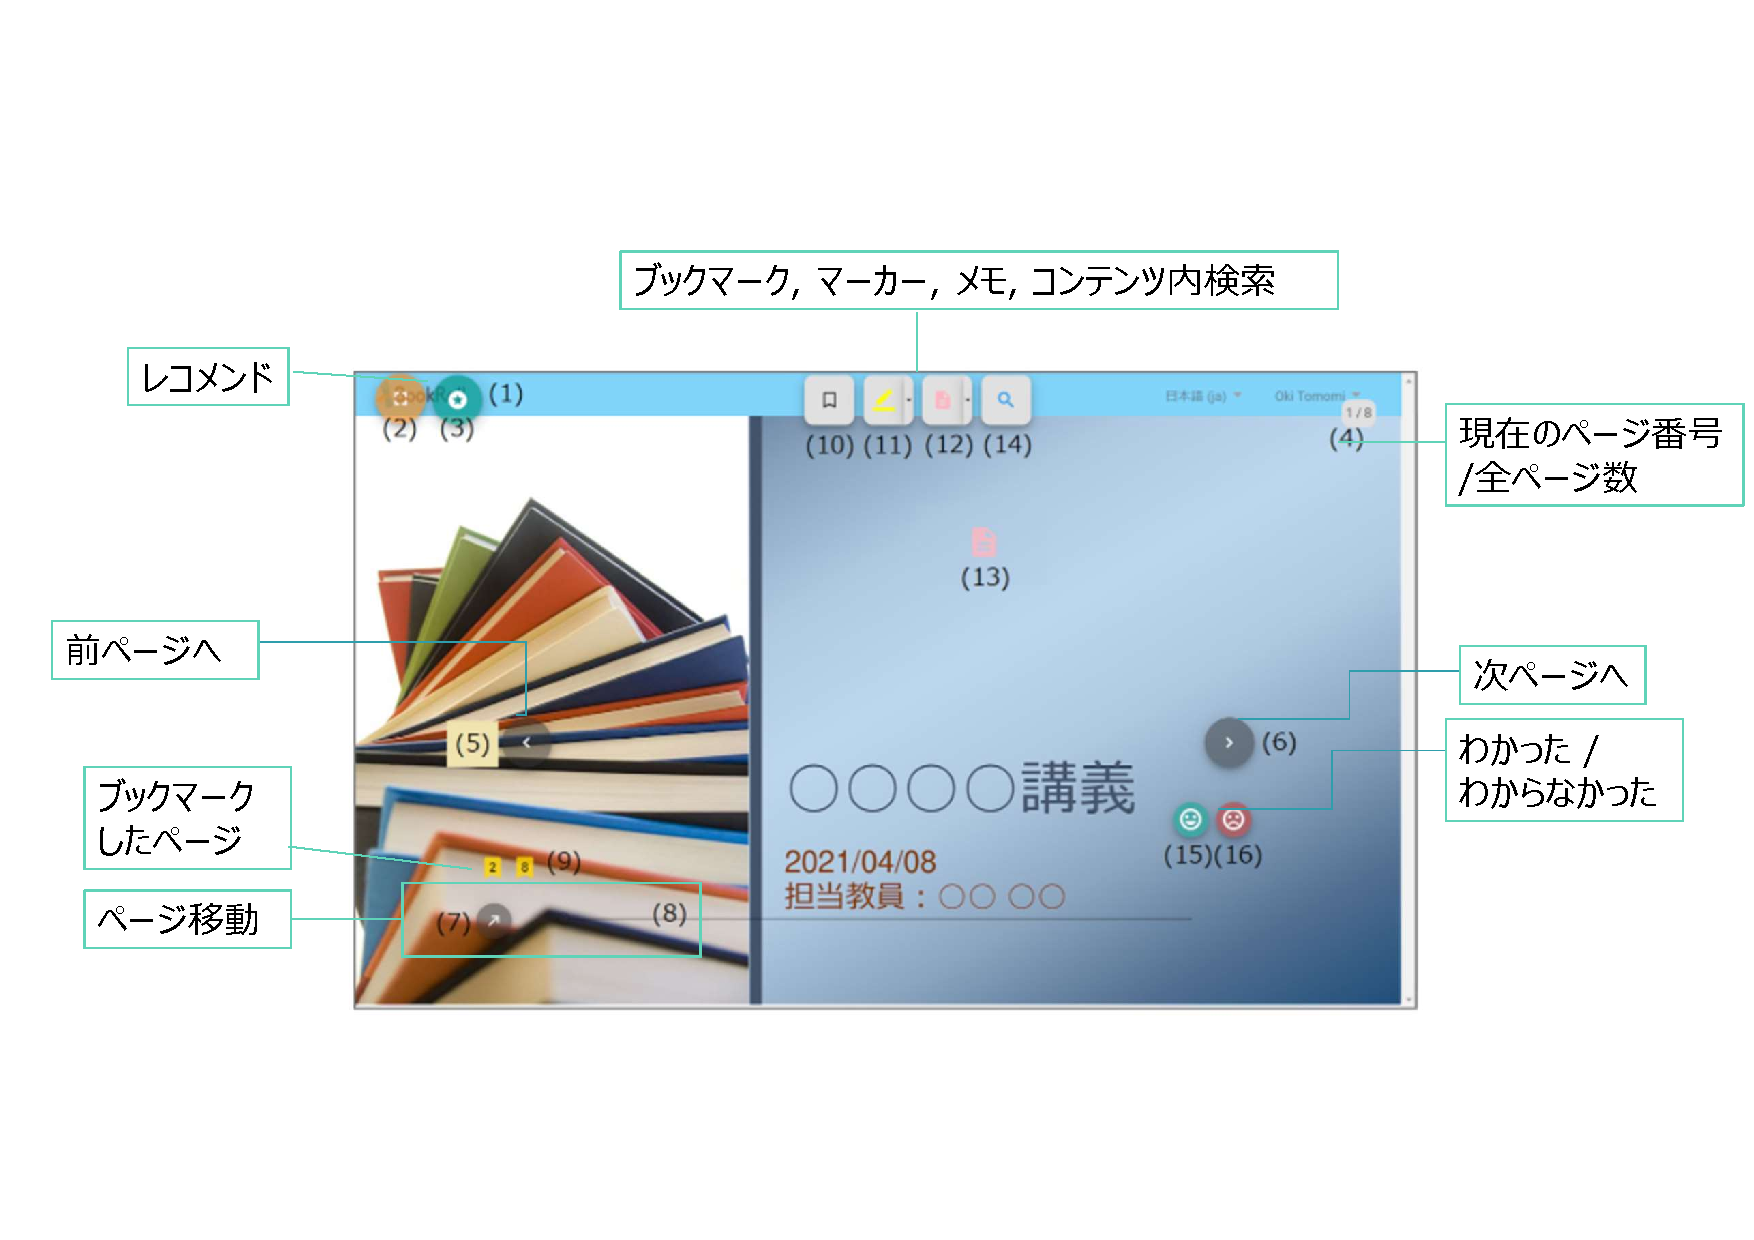
\includegraphics[scale = 0.3]{BookRoll.pdf}
  \caption{BookRollシステム操作画面例}
  \label{fig:BookRollシステム操作画面例}
\end{figure}

閲覧データはコンテンツを開く,閉じる,スライドの遷移などの行動が行われたタイミングで操作を行った学生のID,タイムスタンプ,コンテンツ番号,ページ番号,どのような操作を行ったか等の情報が記録される.記録される主な内容を表1に示す.閲覧データに記録される操作の一部を表2に示す.

\begin{table}[h]
  \centering
  \begin{tabular}{c|l}
    記録名 & 内容 \\ \hline
    contents\_id/name & コンテンツID/名 \\ 
    marker\_position/color & マーカーをつけた場所/色 \\ 
    memo\_text & メモの内容 \\
    operation\_date & 操作した日時 \\ 
    operation\_name & 操作内容 \\ 
    page\_no & 操作したページ \\ 
    userid & 学生に割り振られた番号 \\ \hline
  \end{tabular}
  \caption{記録される主な内容}
  \label{tb:記録される主な内容}
\end{table}

\begin{table*}[h]
  \centering
  \begin{tabular}{c|l}
    operation\_name & 内容 \\ \hline
    OPEN & コンテンツを開く \\ 
    CLOSE & コンテンツを閉じる \\ 
    NEXT & 次のページへ移動 \\
    PREV & ひとつ前のページへ移動 \\ 
    PAGE\_JUMP & 特定のページへ移動 \\ 
    ADD/DELETE BOOKMARK & ブックマークをつける/消す \\
    ADD/DELETE MERKER & マーカーをつける/消す \\
    ADD/DELETE MEMO & メモをつける/消す \\
    SERCH & コンテンツ内検索を行う \\
    GETIT & わかったボタンを押す \\ 
    NOTGETIT & わからなかったボタンを押す \\
    OPEN\_RECOMMENDATION & 関連サイトを開く \\ \hline
  \end{tabular}
  \caption{操作内容の一部}
  \label{tb:操作内容の一部}
\end{table*}

% \section{データ関連の情報・分析結果}


\section{アプローチ}

閲覧データから各スライドにおける各操作回数,各スライドの閲覧時間を,学生ごとに一列のベクトルにして,学生の行動特徴量を求める.
本研究ではこのベクトルで表現される行動特徴量にコンテンツ内容を加えて点数予測を行う方法と小テストに関係するスライドにおける行動だけをとりだして点数予測を行う方法を提案する.
ベースラインとして,行動特徴量のみを使用した場合でも点数予測を行う.
% 行動特徴量として行動回数洗い出す操作は,すべての操作ではなく,OPEN, NEXT, PREV, CLOSE, PAGE\_JUMP, GETIT, OPEN\_RECOMMENDATION, CLOSE\_RECOMMENDATION, NOTGETIT, ADD MARKER, DELETE MARKER, CLICK\_RECOMMENDATION, open\_timeに絞る.

\subsection{手法1:行動特徴量にコンテンツ内容を入れる}

1つ目の提案手法はコンテンツに含まれる文章のベクトル化を行い,そのベクトルを行動特徴量に付け加えて点数予測を行う方法である.現在はベクトル化に事前学習済みのSentence-BERT\cite{sentence-BERT}を使用してスライドごとに768次元のベクトル化を行っている.しかし,スライド内容をベクトル化したものを付け加えただけでは全ての学生が同じベクトルをもつことになるため,スライドベクトルに重みづけを行うことで学生ごとに違ったベクトルを作成する.重みには各スライドの閲覧時間を使用し,学生の閲覧時間が長いスライドほど重要度を高く設定する.ベクトルは各スライドに対し作成されているため,このままでは行動特徴量が大きくなるので,重みづけを行ったベクトルを足し合わせることでベクトルの圧縮を行う.


\subsection{手法2:小テストに関係するスライドにおける行動だけをとりだす}

2つ目の提案手法は小テストに関係するスライドにおける行動だけをとりだし点数予測を行う方法である.小テスト1問ごとに問題文と正解文をSentence-BERTを使用して787次元のベクトル化を行い,小テストベクトルを作成する.小テストベクトルとスライドベクトルとのコサイン類似度を求め,スライドと問のコサイン類似度が0.4以上の値のみを足し合わせ,足し合わせた値を各スライドに対する重要度とする.この重要度を使って各スライドでの行動特徴量に重みづけを行い,新たな行動特徴量とし、これを用いて点数予測を行う.


\section{点数予測・評価}

\subsection{使用データセット}

本研究では,2020年に九州大学で行われた「サイバーセキュリティ基礎論」という講義で使用されたBookRollシステムから得た閲覧データとコンテンツ情報,毎週講義後に行われる小テストから得たデータを使用する.講義は80分講義,10分小テストという形式で100名の学生に対し7週間にわたって行われ,閲覧データは合計200,818ログ記録されている.
小テストは5問の択一式の問題で構成され,小テストデータは学生が小テストを提出したタイミングで記録される.データには問題の文章,学生の選択した選択肢,正解かどうか,提出時間が含まれている.

\subsection{予測・評価方法}
点数予測は小テストごとにLightGBMを使用して行う.5-foldのクロスバリデーションでRSMEを計算し,評価する.
評価には小テストデータから得た,小テストごとに求めた5点満点の点数を使用する.
今回は行動特徴量を講義時間外の行動もすべて含む行動特徴量を使用して点数予測を行った結果と,講義時間内と前後1時間の行動に絞った行動特徴量を使用して点数予測を行った結果をそれぞれ評価し,ベースラインと提案手法を比較する.


\section{結果}

ベースラインの手法と提案手法で点数予測を行った結果のRSMEを示す.図2,図3・表4,表5の横軸のアルファベットと手法との対応を表3に示している.
図2,図3は小テストごとに求めたRMSEの平均をとってグラフにしている.図2,表4は講義時間外のデータも含んで予測した結果,図3,表5は講義時間内と前後1時間に絞ったデータで予測した結果である.図2,図3,表4,表5では講義時間外のデータも含んだ場合で予測した結果を(外),講義時間内と前後1時間に絞ったデータで予測した場合を(内)として表している.
小テストごとの詳しいRMSEの値は表4,表5に示している.2週目は2つのコンテンツが使用され,小テストが2回分行われているため,2週目-1,2週目-2と分けて点数予測を行っている.
表4,表5は色が濃いほどRMSEの値が小さくなっている.


\begin{table}[h]
  \centering
  \begin{tabular}{c|r}
    \hline
    A & ベースライン(講義時間外含む) \\ \hline
    B & 提案手法(手法1講義時間外含む) \\ \hline
    C & 提案手法(手法2講義時間外含む) \\ \hline
    D & ベースライン(講義時間内&前後1時間) \\ \hline
    E & 提案手法(手法1講義時間内&前後1時間) \\ \hline
    F & 提案手法(手法2講義時間内&前後1時間) \\ \hline
  \end{tabular}
  \caption{結果横軸対応表}
  \label{tb:結果横軸対応表}
\end{table}


\begin{figure}[h]
  \centering
  \includegraphics[scale = 0.3]{RMSEmeanv2-1.pdf}
  \caption{小テストごとに求めたRMSEの平均(外)}
  \label{fig:小テストごとに求めたRMSEの平均(外)}
\end{figure}

\begin{figure}[h]
  \centering
  \includegraphics[scale = 0.3]{RMSEmeanv2-2.pdf}
  \caption{小テストごとに求めたRMSEの平均(内)}
  \label{fig:小テストごとに求めたRMSEの平均(内)}
\end{figure}

\begin{table}[h]
  \centering
  \includegraphics[scale = 0.2]{RMSEhyov2-1.pdf}
  \caption{小テストごとに求めたRMSEの平均(外)}
  \label{tb:小テストごとのRMSE(外)}
\end{table}

\begin{table}[h]
  \centering
  \includegraphics[scale = 0.2]{RMSEhyov2-2.pdf}
  \caption{小テストごとに求めたRMSEの平均(内)}
  \label{tb:小テストごとのRMSE(内)}
\end{table}



\section{課題・今後の計画}

結果から,学生の行動を講義時間内(前後1時間含む)に絞ることは点数予測の精度向上に手法によっては繋がる.また,図2のB,図3のEでRMSEの値が下がっていることよりコンテンツ内容を含めることは点数予測の精度向上に繋がり,学習行動の中ではスライドの閲覧時間がより重要になるのではないだろうか.
また,図2のC,図3のFから見られるように手法2ではベースラインとほとんどRMSEの値の変化がなかった.これは各学生に対して全く同じ重みを使用しているためであると考える.これより,行動の重要度及びスライドの重要度によって重みを変えることでより高い精度を期待できるのではないだろうか.

\begin{itemize}
      \item 12~2月: 精度向上を探る・論文執筆・修正・提出
\end{itemize}

\begin{thebibliography}{10}
  \bibitem[1]{yosoku} Sukrit Leelaluk, Tsubasa Minematsu, Yuta Taniguchi, Fumiya Okubo, Atsushi Shimada, Predicting student performance based on Lecture Materials data using Neural Network Models, CEUR Workshop Proceedings, March 21-22, 2022
  \bibitem[2]{BR1}椎野徹也, 峰松翼, 島田敬士, 谷口倫一郎, デジタル教材の学習ログと成績の関連分析, Vol.2020-CLE-30 No.10, 2020/3/9
  \bibitem[3]{sentence-BERT} Nils Reimers and Iryna Gurevych, Sentence-BERT: Sentence Embeddings using Siamese BERT-Networks, Proceedings of the 2019 Conference on Empirical Methods in Natural Language Processingand the 9th International Joint Conference on Natural Language Processing, pages 3982–3992,November 3–7, 2019
\end{thebibliography}
  



\end{document}
